% Fig. 1 — NEMA-Q architecture (component-accounting view).
% Standalone: compile with pdflatex; \includegraphics the resulting PDF,
% or paste the tikzpicture into the sn-jnl document directly.
\documentclass[tikz,border=6pt]{standalone}
\usepackage{amsmath,amssymb}
\usetikzlibrary{positioning,fit,arrows.meta,calc}

\begin{document}
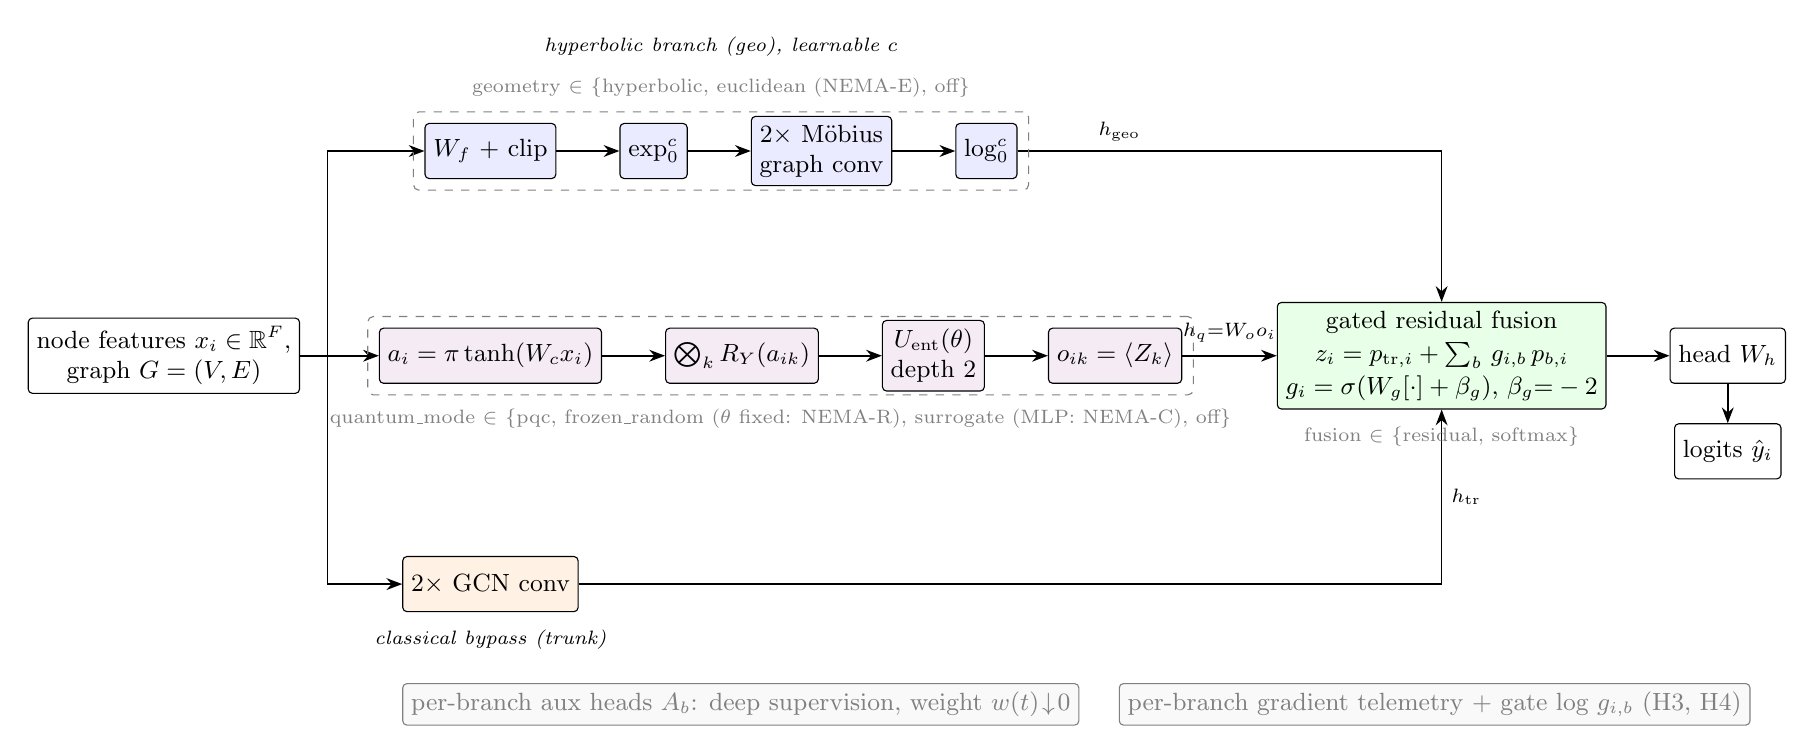
\begin{tikzpicture}[
  font=\small,
  node distance=4mm and 8mm,
  box/.style={draw, rounded corners=1.5pt, align=center, minimum height=7mm,
              inner sep=3pt, fill=white},
  geo/.style={box, fill=blue!8},
  qua/.style={box, fill=violet!8},
  cla/.style={box, fill=orange!10},
  fus/.style={box, fill=green!9},
  aux/.style={box, draw=gray, text=gray, fill=gray!5, minimum height=5mm},
  swap/.style={draw=gray, dashed, rounded corners=2pt, inner sep=4pt},
  swaplab/.style={gray, font=\scriptsize, align=center},
  arr/.style={-{Stealth[length=2mm]}, semithick},
  lab/.style={font=\scriptsize\itshape, align=center}
]

% ---------------- q branch (middle row, y=0) ----------------
\node[qua] (qcomp) at (3.2,0) {$a_i=\pi\tanh(W_c x_i)$};
\node[qua, right=of qcomp] (qemb) {$\bigotimes_k R_Y(a_{ik})$};
\node[qua, right=of qemb] (qsel) {$U_{\mathrm{ent}}(\theta)$\\ depth 2};
\node[qua, right=of qsel] (qobs) {$o_{ik}=\langle Z_k\rangle$};

% ---------------- input ----------------
\node[box, left=10mm of qcomp] (input)
  {node features $x_i \in \mathbb{R}^F$,\\ graph $G=(V,E)$};

% ---------------- geo branch (top row) ----------------
\node[geo] (geocomp) at (3.2,2.6) {$W_f$ + clip};
\node[geo, right=of geocomp] (geoexp) {$\exp_0^c$};
\node[geo, right=of geoexp] (geoconv) {$2\times$ M\"obius\\ graph conv};
\node[geo, right=of geoconv] (geolog) {$\log_0^c$};

% ---------------- trunk (bottom row) ----------------
\node[cla] (trunk) at (3.2,-2.9) {$2\times$ GCN conv};
\node[lab, below=1mm of trunk.south] {classical bypass (trunk)};

% ---------------- fusion + head ----------------
\node[fus, right=12mm of qobs] (fusion)
  {gated residual fusion\\[1pt]
   $z_i = p_{\mathrm{tr},i} + \sum_{b}\, g_{i,b}\, p_{b,i}$\\[1pt]
   $g_i=\sigma(W_g[\cdot]+\beta_g)$, $\beta_g{=}-2$};
\node[box, right=of fusion] (head) {head $W_h$};
\node[box, below=5mm of head] (out) {logits $\hat y_i$};

% ---------------- arrows ----------------
\draw[arr] (input.east) -- ++(3.5mm,0) |- (geocomp.west);
\draw[arr] (input.east) -- (qcomp.west);
\draw[arr] (input.east) -- ++(3.5mm,0) |- (trunk.west);
\draw[arr] (geocomp) -- (geoexp);
\draw[arr] (geoexp) -- (geoconv);
\draw[arr] (geoconv) -- (geolog);
\draw[arr] (qcomp) -- (qemb);
\draw[arr] (qemb) -- (qsel);
\draw[arr] (qsel) -- (qobs);
\draw[arr] (geolog.east) -| node[pos=0.12, above, font=\scriptsize] {$h_{\mathrm{geo}}$}
  (fusion.north);
\draw[arr] (qobs.east) -- node[above=0.5mm, font=\scriptsize] {$h_q{=}W_o o_i$} (fusion.west);
\draw[arr] (trunk.east) -| node[pos=0.75, right, font=\scriptsize] {$h_{\mathrm{tr}}$}
  (fusion.south);
\draw[arr] (fusion) -- (head);
\draw[arr] (head) -- (out);

% ---------------- swap boxes + labels ----------------
\node[swap, fit=(geocomp)(geolog)] (geoswap) {};
\node[swaplab, anchor=south] (geoswaplab) at ($(geoswap.north)+(0,0.5mm)$)
  {geometry $\in$ \{hyperbolic, euclidean (NEMA-E), off\}};
\node[lab, anchor=south] at ($(geoswaplab.north)+(0,0.3mm)$)
  {hyperbolic branch (geo), learnable $c$};
\node[swap, fit=(qcomp)(qobs)] (qswap) {};
\node[swaplab, anchor=north] at ($(qswap.south)+(0,-0.5mm)$)
  {quantum\_mode $\in$ \{pqc, frozen\_random ($\theta$ fixed: NEMA-R),
   surrogate (MLP: NEMA-C), off\}};
\node[swaplab, anchor=north] at ($(fusion.south)+(0,-1mm)$)
  {fusion $\in$ \{residual, softmax\}};

% ---------------- annotation legend (bottom) ----------------
\node[aux, anchor=north west] at ($(trunk.south west)+(0,-9mm)$) (auxheads)
  {per-branch aux heads $A_b$: deep supervision, weight $w(t)\!\downarrow\!0$};
\node[aux, right=5mm of auxheads] (telemetry)
  {per-branch gradient telemetry + gate log $g_{i,b}$ (H3, H4)};

\end{tikzpicture}
\end{document}
